% SOURCE_AUTHORITY: sga5_fr_workpass.tex, lines 2143--2310 (LF-normalized unit).
% SOURCE_SHA256: 791F4EFFC5E02832D5D77ED03518C8156D6F07E4C8238B03545DB93D883FBB28
\subsection*{Proposição 2.5}
O diagrama 2.5.1 seguinte, cujo quadrado da direita se deduz de 2.4.1 aplicando $\uRHom$ no sentido de 2.1.3 e 2.1.5, é comutativo:
\begin{equation}\tag{2.5.1}
\resizebox{0.98\textwidth}{!}{%
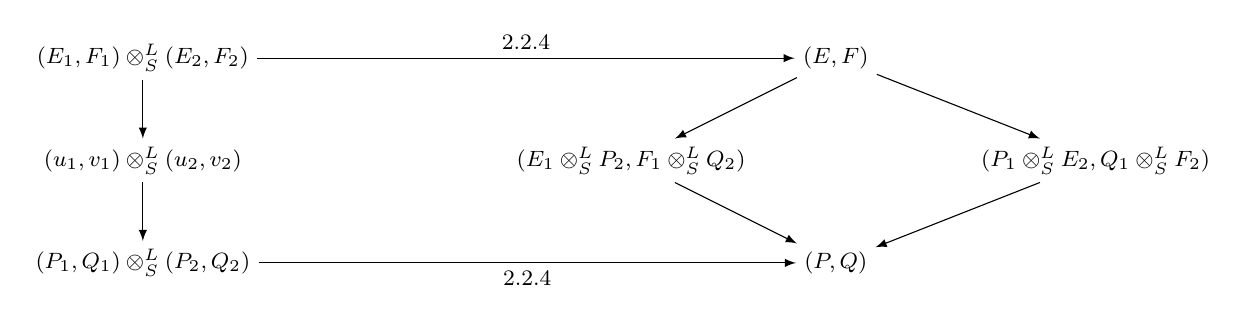
\begin{tikzpicture}[>=latex,baseline=(current bounding box.center)]
\footnotesize
\node (A) at (0,2.6) {$\uRHom(E_1,F_1)\otimes^L_S\uRHom(E_2,F_2)$};
\node (B) at (0,1.3) {$\uRHom(u_1,v_1)\otimes^L_S\uRHom(u_2,v_2)$};
\node (C) at (0,0) {$\uRHom(P_1,Q_1)\otimes^L_S\uRHom(P_2,Q_2)$};
\node (D) at (8.8,2.6) {$\uRHom(E,F)$};
\node (E) at (6.2,1.3) {$\uRHom(E_1\otimes^L_SP_2,F_1\otimes^L_SQ_2)$};
\node (F) at (12.1,1.3) {$\uRHom(P_1\otimes^L_SE_2,Q_1\otimes^L_SF_2)$};
\node (G) at (8.8,0) {$\uRHom(P,Q)$};
\draw[->] (A) -- node[above] {$2.2.4$} (D);
\draw[->] (A) -- (B);
\draw[->] (B) -- (C);
\draw[->] (C) -- node[below] {$2.2.4$} (G);
\draw[->] (D) -- (E);
\draw[->] (D) -- (F);
\draw[->] (E) -- (G);
\draw[->] (F) -- (G);
\end{tikzpicture}}
\end{equation}

\subsection*{2.6}
A demonstração de 2.5 ocupará o restante do n\textsuperscript{o}~2. Deduz-se de 1.6.3 que, se $w_i:L_i\to M_i$ for uma flecha de tipo~1 sobre $f_i$, a flecha $w=w_1\otimes^{L}_{S}w_2$ tornará comutativo o diagrama
\[
\begin{tikzcd}[column sep=large,row sep=large]
& L_1\otimes^L_S L_2 \arrow[dl,"{L_1\otimes^L_S w_2}"'] \arrow[dr,"{w_1\otimes^L_S L_2}"] & \\
L_1\otimes^L_S M_2 \arrow[dr,"{w_1\otimes^L_S M_2}"'] & & M_1\otimes^L_S L_2 \arrow[dl,"{M_1\otimes^L_S w_2}"]\\
& M_1\otimes^L_S M_2 & .
\end{tikzcd}
\]
Aplicando essa observação a $w_i=\uRHom(u_i,v_i)$, vê-se que basta demonstrar os seguintes casos particulares de 2.5.

\subsection*{Corolário 2.6.1}
Sejam $f:X\to Y$ um $S$-morfismo, $S'$ um $S$-esquema, $f':X'\to Y'$ o morfismo deduzido de $f$ pela mudança de base $S'\to S$, $E,F\in\ob D_{\ctf}(X)$, $P,Q\in\ob D_{\ctf}(Y)$, $P',Q'\in\ob D_{\ctf}(S')$, $(u,v)\in\Hom_f^{(2,1)}((E,F),(P,Q))$ (resp. $\Hom_f^{(3,4)}((E,F),(P,Q))$). Tem-se então um quadrado comutativo, cujas flechas verticais são de tipo~1 sobre $f'$:
\begin{equation}\tag{2.6.1.1}
\begin{tikzcd}[column sep=large,row sep=large]
\uRHom(E,F)\otimes^L_S\uRHom(P',Q') \arrow[r,"2.2.4"] \arrow[d,"{\uRHom(u,v)\otimes^L_S\uRHom(P',Q')}"'] & \uRHom(E\otimes^L_SP',F\otimes^L_SQ') \arrow[d,"{\uRHom(u\otimes^L_SP',v\otimes^L_SQ')}"]\\
\uRHom(P,Q)\otimes^L_S\uRHom(P',Q') \arrow[r,"2.2.4"'] & \uRHom(P\otimes^L_SP',Q\otimes^L_SQ').
\end{tikzcd}
\end{equation}
Examinemos primeiro o caso em que $(u,v)$ é de tipo $(2,1)$. Por funtorialidade, podemos supor que $E=f^{*}P$, $F=f^{*}Q$, e que $(u,v)$ seja dado pela identidade de $(f^{*}P,f^{*}Q)$. A comutatividade de 2.6.1.1 no caso $P'=Q'=A_{S'}$ é evidente; para estabelecê-la no caso geral, basta, portanto, verificar que, para $L,M\in\ob D_{\ctf}(Y)$, o quadrado
\[
\begin{tikzcd}[column sep=large,row sep=large]
f^{*}\uRHom(E,F)\otimes^L f^{*}\uRHom(L,M) \arrow[r,"{f^*(2.2.3)}"] \arrow[d,"{2.1.1\otimes 2.1.1}"'] & f^{*}\uRHom(E\otimes^LL,F\otimes^LM) \arrow[d,"2.1.1"]\\
\uRHom(f^{*}E,f^{*}F)\otimes^L\uRHom(f^{*}L,f^{*}M) \arrow[r,"2.2.3"'] & \uRHom(f^{*}(E\otimes^LL),f^{*}(F\otimes^LM))
\end{tikzcd}
\]
é comutativo. Ora, verifica-se imediatamente que as duas compostas desse quadrado são adjuntas do produto tensorial das flechas de avaliação
\[
f^{*}E\otimes^L f^{*}\uRHom(E,F)\longrightarrow f^{*}F
\quad\text{e}\quad
f^{*}L\otimes^L f^{*}\uRHom(L,M)\longrightarrow f^{*}M,
\]
de onde resulta a afirmação.

\enlargethispage{-2\baselineskip}
Passemos agora ao caso em que $(u,v)$ é de tipo $(3,4)$. Por funtorialidade, podemos supor que $P=f_{!}E$, $F=f^{!}Q$, e que $(u,v)$ seja definido por $(\Id_P,\Id_F)$. Devemos demonstrar a comutatividade do quadrado
\[
\begin{tikzcd}[column sep=large,row sep=large]
f_*\uRHom(E,f^!Q)\otimes^L_S\uRHom(P',Q') \arrow[r,"b"] \arrow[d,"{a\otimes^L_S\uRHom(P',Q')}"'] & f'_*\uRHom(E\otimes^L_SP',f^!Q\otimes^L_SQ') \arrow[d,"a'"]\\
\uRHom(f_!E,Q)\otimes^L_S\uRHom(P',Q') \arrow[r,"2.2.4"'] & \uRHom(f_!E\otimes^L_SP',Q\otimes^L_SQ'),
\end{tikzcd}
\]
onde $b$ é a composta de $f'_*(2.2.4)$ e de um isomorfismo de mudança de base, $a$ é o isomorfismo de dualidade (SGA~4~XVIII~3.1.9.6), e $a'$ é a composta do isomorfismo de dualidade (relativo a $E\otimes^L_SP'$ e $Q\otimes^L_SQ'$) e dos isomorfismos de mudança de base
\[
f_!E\otimes^L_SP'\xrightarrow[\sim]{c}f'_!(E\otimes^L_SP'),
\qquad
f^!Q\otimes^L_SQ'\xrightarrow[\sim]{d}f'^!(Q\otimes^L_SQ').
\]
Recordemos que $a$ é a composta da flecha canônica (SGA~4~XVIII~3.1.9.5)
\[
f_*\uRHom(E,f^!Q)\longrightarrow\uRHom(f_!E,f_!f^!Q)
\]
e da flecha definida pela flecha de adjunção $f_!f^!Q\to Q$. Tem-se uma descrição análoga de $a'$, como composta da flecha citada
\begin{equation}\tag{*}
f'_*\uRHom(E\otimes^L_SP',f^!Q\otimes^L_SQ')\longrightarrow
\uRHom(f'_!(E\otimes^L_SP'),f'_!(f^!Q\otimes^L_SQ')),
\end{equation}
das flechas definidas por $c$ e $d$ e da flecha definida pela flecha de adjunção
\[
f'_!f'^!(Q\otimes^L_SQ')\longrightarrow Q\otimes^L_SQ'.
\]
Ora, por definição, $d$ é adjunta da flecha
\[
f'_!(f^!Q\otimes^L_SQ')\longrightarrow Q\otimes^L_SQ'
\]
definida pelo isomorfismo de mudança de base $f'_!(f^!Q\otimes^L_SQ')\simeq f_!f^!Q\otimes^L_SQ'$ e pela flecha de adjunção $f_!f^!Q\to Q$; em outras palavras, o quadrado
\[
\begin{tikzcd}[column sep=large,row sep=large]
f'_!(f^!Q\otimes^L_SQ') \arrow[r,"{f'_!d}"] \arrow[d,"{\text{camb. de base}\ \sim}"'] & f'_!f'^!(Q\otimes^L_SQ') \arrow[d,"\mathrm{adj}"]\\
f_!f^!Q\otimes^L_SQ' \arrow[r,"{\mathrm{adj}\otimes 1}"'] & Q\otimes^L_SQ'
\end{tikzcd}
\]
é comutativo. Consequentemente, $a'$ também pode ser descrita como composta de $(*)$, da flecha definida por $c$ e das definidas pelo isomorfismo de mudança de base
\[
f'_!(f^!Q\otimes^L_SQ')\xrightarrow{\sim}f_!f^!Q\otimes^L_SQ'
\]
e a flecha de adjunção $f_!f^!Q\to Q$. Esta decomposição de $a'$ e $a$ dada acima, juntamente com a comutabilidade do quadrado
\[
\begin{tikzcd}[column sep=large,row sep=large]
\uRHom(f_!E,f_!f^!Q)\otimes^L_S\uRHom(P',Q') \arrow[r] \arrow[d] & \uRHom(f_!E\otimes^L_SP',f_!f^!Q\otimes^L_SQ') \arrow[d]\\
\uRHom(f_!E,Q)\otimes^L_S\uRHom(P',Q') \arrow[r] & \uRHom(f_!E\otimes^L_SP',Q\otimes^L_SQ'),
\end{tikzcd}
\]
definido por 2.2.4 e pela flecha de adjunção $f_!f^!Q\to Q$, mostram que, para estabelecer a comutatividade de 2.6.2, basta demonstrar a compatibilidade seguinte.

\subsection*{Lema 2.6.3}
Sejam $f$, $f'$, $E$, $F$, $P'$, $Q'$ como em 2.6.1. Tem-se então um quadrado comutativo
\[
\begin{tikzcd}[column sep=large,row sep=large]
f_*\uRHom(E,F)\otimes^L_S\uRHom(P',Q') \arrow[r,"(1)"] \arrow[d,"(2)"'] & f'_*\uRHom(E\otimes^L_SP',F\otimes^L_SQ') \arrow[d,"(4)"]\\
\uRHom(f_!E,f_!F)\otimes^L_S\uRHom(P',Q') \arrow[r,"(3)"'] & \uRHom(f_!E\otimes^L_SP',f_!F\otimes^L_SQ'),
\end{tikzcd}
\]
onde (1) é a composição do isomorfismo de mudança de base
\[
f_*\uRHom(E,F)\otimes^L_S -\xrightarrow{\sim}f'_*\bigl(\uRHom(E,F)\otimes^L_S-\bigr)
\]
e de $f'_*(2.2.4)$; (2) deduz-se da flecha canônica
\[
f_*\uRHom(E,F)\longrightarrow\uRHom(f_!E,f_!F)
\]
(SGA~4~XVIII~3.1.9.5) aplicando $\otimes^L_S\uRHom(P',Q')$; (3) é dada por 2.2.4; finalmente, (4) é a composta da flecha canônica
\[
f'_*\uRHom(E\otimes^L_SP',F\otimes^L_SQ')
\longrightarrow
\uRHom(f'_!(E\otimes^L_SP'),f'_!(F\otimes^L_SQ'))
\]
(loc. cit.) e das flechas definidas pelos isomorfismos de mudança de base
\[
f'_!(E\otimes^L_SP')\xrightarrow{\sim}f_!E\otimes^L_SP',
\qquad
f'_!(F\otimes^L_SQ')\xrightarrow{\sim}f_!F\otimes^L_SQ'.
\]
Voltando à definição da flecha (SGA~4~XVIII~3.1.9.5), escolhemos uma compactificação de $f$\footnote{A flecha citada define-se mediante tal compactificação, mas não depende dela: esse ponto, tacitamente admitido em (loc. cit.), verifica-se facilmente.}, e reduzimo-nos a demonstrar o lema separadamente no caso em que $f$ é uma imersão aberta e naquele em que $f$ é um morfismo próprio.

\emph{a) Caso em que $f$ é uma imersão aberta.} Por adjunção (2.2.1), basta ver que, se tensorizarmos o quadrado de 2.6.3 por $f_!E\otimes^L_SP'$ e o compusermos com a flecha de avaliação 2.2.2
\[
(f_!E\otimes^L_SP')\otimes^L\uRHom(f_!E\otimes^L_SP',f_!F\otimes^L_SQ')\longrightarrow f_!F\otimes^L_SQ',
\]
o quadrado obtido será comutativo. Ora, os vértices desse quadrado são nulos fora de $X'$, de modo que basta verificar que o quadrado induzido sobre $X'$ comuta, o que é trivial.

\emph{b) Caso em que $f$ é um morfismo próprio.} Tem-se então $f_!=f_*$, $f'_!=f'_*$. Vê-se facilmente que a composta de
\[
f_*\uRHom(E,F)\longrightarrow\uRHom(f_*E,f_*F)
\]
com o isomorfismo de dualidade trivial
\[
\uRHom(f_*E,f_*F)\xrightarrow{\sim}f_*\uRHom(f^{*}f_*E,F)
\]
(2.1.4) é apenas a flecha deduzida da flecha de adjunção $f^{*}f_*E\to E$ aplicando $f_*\uRHom(-,F)$. Da mesma forma, a composição de (4) com o isomorfismo de dualidade trivial
\[
\uRHom(f_*E\otimes^L_SP',f_*F\otimes^L_SQ')\xrightarrow{\sim}f'_*\uRHom(f^{*}f_*E\otimes^L_SP',F\otimes^L_SQ')
\]
(identificando-se $f_*F\otimes^L_SQ'$ com $f'_*(F\otimes^L_SQ')$ mediante o isomorfismo canônico) não é senão a flecha deduzida da flecha de adjunção $f^{*}f_*E\to E$ aplicando $f'_*\uRHom(-\otimes^L_SP',F\otimes^L_SQ')$. Reduzimo-nos, portanto, a verificar a comutatividade do quadrado
\[
\begin{tikzcd}[column sep=large,row sep=large]
\uRHom(f_*E,f_*F)\otimes^L_S\uRHom(P',Q') \arrow[r,"(3)"] \arrow[d] & \uRHom(f_*E\otimes^L_SP',f_*F\otimes^L_SQ') \arrow[d]\\
f_*\uRHom(f^{*}f_*E,F)\otimes^L_S\uRHom(P',Q') \arrow[r,"(1')"'] & f'_*\uRHom(f^{*}f_*E\otimes^L_SP',F\otimes^L_SQ'),
\end{tikzcd}
\]
onde as flechas verticais são os isomorfismos de dualidade trivial e $(1')$ é $(1)$ com $E$ substituído por $f^{*}f_*E$. Mas essa comutatividade é um caso particular da de 2.6.1.1 no caso, já tratado, em que $(u,v)$ é de tipo $(2,1)$ (tomar $u:f^{*}f_*E\to f_*E$ dado pela identidade de $f^{*}f_*E$, e $v:F\to f_*F$ dado pela identidade de $f_*F$). Demonstramos, portanto, 2.6.3. Como vimos, daí resulta a comutatividade de 2.6.2, o que conclui a demonstração de 2.6.1 e, finalmente, de 2.5.

\clearpage
\section{Correspondências cohomológicas}
